\chapter{Spatial Arrangement}
\label{ch:spatial_arrangement}

%%%%%%%%%%%%%%%%%%
\section{Overview}
Refer to the introduction for algorithm explanation
[ref. \ref{ch:arrangement_algorithm}].

@O lib/jl/spatial_arrangement.jl
@{@< spatial\_arrangement support functions @>


function spatial_arrangement(V::Verts, EV::Cells, FE::Cells; multiproc=false)
    fs_num = size(FE, 1)
    sp_idx = spatial_index(V, EV, FE)

    rV = Verts(0,3)
    rEV = spzeros(Int8,0,0)
    rFE = spzeros(Int8,0,0)

    if (multiproc == true)
        @< Run parallel spatial\_arrangement @>
    else
        @< Run sequential spatial\_arrangement @>
    end

    rV, rEV, rFE = merge_vertices(rV, rEV, rFE)

    @< Create 3-cells @>

    return rV, rEV, rFE, rCF
end

@}

%+++++++++++++++++++++++++++++%
\subsection{Tests and examples}

Unit tests has yet to be written for this chapter, but general
examples are available at the end of the chapter [ref. \ref{sec:spatial_arrangement_examples}]




%%%%%%%%%%%%%%%%%%%%%%%%%%%
\section{Parallel approach}

If the user does not require parallelization 
(using the \texttt{multiproc} argument) the sequential version
of the implementation starts. This fragments each face sequentially.

@D Run sequential spatial\_arrangement
@{for sigma in 1:fs_num
    print(sigma, "/", fs_num, "\r")
    nV, nEV, nFE = frag_face(V, EV, FE, sp_idx, sigma)
    rV, rEV, rFE = skel_merge(rV, rEV, rFE, nV, nEV, nFE)
end
@}

If instead, parallelization is required, we build the in and out channels,
we feed the data to the input channel, we dispatch tasks to the workers and then
read the data from the output channel. We also defined a function
called \texttt{frag\_face\_channel} to call the \texttt{frag\_face} function
from every worker with the data inside the output channel.

@D Run parallel spatial\_arrangement
@{in_chan = RemoteChannel(()->Channel{Int64}(0))
out_chan = RemoteChannel(()->Channel{Tuple}(0))

@@schedule begin
    for sigma in 1:fs_num
        put!(in_chan, sigma)
    end
    for p in workers()
        put!(in_chan, -1)
    end
end

for p in workers()
    @@async Base.remote_do(
        frag_face_channel, p, in_chan, out_chan, V, EV, FE, sp_idx)
end

for sigma in 1:fs_num
    rV, rEV, rFE = skel_merge(rV, rEV, rFE, take!(out_chan)...)
end
@}

@D spatial\_arrangement support functions
@{function frag_face_channel(in_chan, out_chan, V, EV, FE, sp_idx)
    run_loop = true
    while run_loop
        sigma = take!(in_chan)
        if sigma != -1
            put!(out_chan, frag_face(V, EV, FE, sp_idx, sigma))
        else
            run_loop = false
        end
    end
end
@}




%%%%%%%%%%%%%%%%%%%%%%%%%%%%%
\section{Face fragmentation}

To fragment a $\sigma$ 2-cell, we flat it out on the $x_3=0$ plane,
we launch the planar arrangement and then bring the fragmented $\sigma$
to its original place.

@D spatial\_arrangement support functions
@{function frag_face(V, EV, FE, sp_idx, sigma)
    vs_num = size(V, 1)

    sigmavs = (abs.(FE[sigma:sigma,:])*abs.(EV))[1,:].nzind 
    sV = V[sigmavs, :]
    sEV = EV[FE[sigma, :].nzind, sigmavs]

    @< Sigma flattening @>

    nV, nEV, nFE = planar_arrangement(sV, sEV, sparsevec(ones(Int8, length(sigmavs))))

    if nV == nothing
        return [], spzeros(Int8, 0,0), spzeros(Int8, 0,0)
    end

    nvsize = size(nV, 1)
    nV = [nV zeros(nvsize) ones(nvsize)]*inv(M)[:, 1:3]
    return nV, nEV, nFE
end
@}

To flattening of $\sigma$ on the $x_3=0$ plane,
is performed by building a linear transformation matrix with the
\texttt{submanifold\_mapping} utility [ref. \ref{sec:submanifold_mapping}],
transforming the geometry and intersecting every cell in $\mathcal{I}(\sigma)$
[ref. \ref{sec:spatial_arrangement_overview}]
with the $x_3=0$ plane using \texttt{face\_int} [ref. \ref{sec:face_int}].

@D Sigma flattening
@{M = submanifold_mapping(sV)
tV = ([V ones(vs_num)]*M)[:, 1:3]

sV = tV[sigmavs, :]

for i in sp_idx[sigma]
    tmpV, tmpEV = face_int(tV, EV, FE[i, :])
    
    sV, sEV = skel_merge(sV, sEV, tmpV, tmpEV)
end

sV = sV[:, 1:2]
@}




%%%%%%%%%%%%%%%%%%%%%%%%%%%%%%%%%%%
\section{Coincident vertices merge}
\label{sec:3D_merge_vertices}

The merge of coincident is done in the \texttt{merge\_vertices}
function.

@D spatial\_arrangement support functions
@{function merge_vertices(V::Verts, EV::Cells, FE::Cells, err=1e-4)
    vertsnum = size(V, 1)
    edgenum = size(EV, 1)
    facenum = size(FE, 1)
    newverts = zeros(Int, vertsnum)
    kdtree = KDTree(V')

    @< Find coincident vertices @>
    @< Merge edges @>
    @< Merge faces @>

    return nV, nEV, nFE
end
@}

First of all we need to find vertices which are near enough
to be considered coincident. We perform this operation
relying on the \texttt{NearestNeighbors.jl} package\cite{NearestNeighbors}
which provides a rather good implementation of the \texttt{KDTree} data structure.

So, we identify the vertices to delete and we store a map
from original vertices to new vertices. In the meanwhile
we built a list of vertices to delete and we delete them 
as soon as possible.

@D LAR imports
@{using NearestNeighbors
@}

@D Find coincident vertices
@{todelete = []

i = 1
for vi in 1:vertsnum
    if !(vi in todelete)
        nearvs = inrange(kdtree, V[vi, :], err)

        newverts[nearvs] = i

        nearvs = setdiff(nearvs, vi)
        todelete = union(todelete, nearvs)

        i = i + 1
    end
end

nV = V[setdiff(collect(1:vertsnum), todelete), :]
@}

To delete the edges we write them as couples of vertex
indices. We keep them in two versions: in \texttt{edges}
we put the edges described with the indexes of the new vertices
and in \texttt{oedges} we put the edges relative to the original vertex
indices (we will use them when merging faces). Once we "translated"
the edges, we delete the duplicates (using a set union) and the
degenerated edges. Lastly we build a new EV matrix 
(called \texttt{nEV}). While we
build the matrix, we also build a dictionary which maps edges expressed
as couples of vertex indices into edge indices relative to \texttt{nEV};
this data will be used in the $d=2$ version of this function 
[ref. \ref{sec:2D_merge_vertices}].

@D Merge edges
@{edges = Array{Tuple{Int, Int}, 1}(edgenum)
oedges = Array{Tuple{Int, Int}, 1}(edgenum)

for ei in 1:edgenum
    v1, v2 = EV[ei, :].nzind
    
    edges[ei] = Tuple{Int, Int}(sort([newverts[v1], newverts[v2]]))
    oedges[ei] = Tuple{Int, Int}(sort([v1, v2]))

end
nedges = union(edges)
nedges = filter(t->t[1]!=t[2], nedges)

nedgenum = length(nedges)
nEV = spzeros(Int8, nedgenum, size(nV, 1))

etuple2idx = Dict{Tuple{Int, Int}, Int}()

for ei in 1:nedgenum
    nEV[ei, collect(nedges[ei])] = 1
    etuple2idx[nedges[ei]] = ei
end
@}

To merge the faces, we convert them into a lists of
edges (represented as a couple of vertices). We then remove duplicated faces
by checking which faces use the same vertices. At the end, we use the
maps built during vertices and edges merge to rebuild the \texttt{FE}
matrix correctly using the new vertex indices.

@D Merge faces
@{faces = [[
    map(x->newverts[x], FE[fi, ei] > 0 ? oedges[ei] : reverse(oedges[ei]))
    for ei in FE[fi, :].nzind
] for fi in 1:facenum]


visited = []
function filter_fn(face)

    verts = []
    map(e->verts = union(verts, collect(e)), face)
    verts = Set(verts)

    if !(verts in visited)
        push!(visited, verts)
        return true
    end
    return false
end

nfaces = filter(filter_fn, faces)

nfacenum = length(nfaces)
nFE = spzeros(Int8, nfacenum, size(nEV, 1))

for fi in 1:nfacenum
    for edge in nfaces[fi]
        ei = etuple2idx[Tuple{Int, Int}(sort(collect(edge)))]
        nFE[fi, ei] = sign(edge[2] - edge[1])
    end
end
@}




%%%%%%%%%%%%%%%%%%%%%%%%%%%%%%%%%%%
\section{$3$-cells creation}

@D Create 3-cells
@{@< Compute connected components @>
@< Compute containment tree @>
@< Cell union @>

rCF = minimal_3cycles(rV, rEV, rFE)
@}


%%%%%%%%%%%%%%%%%%%%%%%%
\section{General examples}
\label{sec:spatial_arrangement_examples}

We used this test a lot during development. It builds
a cube made of $3 \times 3 \times 3$ cubes. The it arranges
the cubes, building a sort of Rubik's cube. Then it duplicates
it and rotates a copy by $\pi / 6$ on the $x_1$-axis
and then on the $x_3$-axis.

@D spatial\_arrangement general examples
@{function rubiks_example(ncubes = 3)
    V = Float64[
        0 0 0; 0 1 0;
        1 1 0; 1 0 0;
        0 0 1; 0 1 1;
        1 1 1; 1 0 1
    ]

    EV = sparse(Int8[
        -1  1  0  0  0  0  0  0;
        0 -1  1  0  0  0  0  0;
        0  0 -1  1  0  0  0  0;
        -1  0  0  1  0  0  0  0;
        -1  0  0  0  1  0  0  0;
        0 -1  0  0  0  1  0  0;
        0  0 -1  0  0  0  1  0;
        0  0  0 -1  0  0  0  1;
        0  0  0  0 -1  1  0  0;
        0  0  0  0  0 -1  1  0;
        0  0  0  0  0  0 -1  1;
        0  0  0  0 -1  0  0  1;
    ])

    FE = sparse(Int8[
        1  1  1 -1  0  0  0  0  0  0  0  0;
        0  0  0  0  0  0  0  0 -1 -1 -1  1;
        -1  0  0  0  1 -1  0  0  1  0  0  0;
        0 -1  0  0  0  1 -1  0  0  1  0  0;
        0  0 -1  0  0  0  1 -1  0  0  1  0;
        0  0  0  1 -1  0  0  1  0  0  0 -1;
    ])

    cube = [V, EV, FE]
    cubesRow = (zeros(0,3),spzeros(Int8,0,0),spzeros(Int8,0,0))

    for i in 1:ncubes
        cubesRow = LARLIB.skel_merge(cubesRow..., cube...)
        cube[1] = cube[1] + [zeros(8) zeros(8) ones(8)]
    end

    cubesRow = collect(cubesRow)
    cubesPlane = cubesRow
    num = size(cubesRow[1], 1)
    for i in 1:ncubes
        cubesPlane = LARLIB.skel_merge(cubesPlane..., cubesRow...)
        cubesRow[1] = cubesRow[1] + [zeros(num) ones(num) zeros(num)]
    end

    cubesPlane = collect(cubesPlane)
    cubesCube = cubesPlane
    num = size(cubesPlane[1], 1)
    for i in 1:ncubes
        cubesCube = LARLIB.skel_merge(cubesCube..., cubesPlane...)
        cubesPlane[1] = cubesPlane[1] + [ones(num) zeros(num) zeros(num)]
    end

    println("Arranging a cube of ", ncubes^3," cubes...")
    rubik = LARLIB.spatial_arrangement(cubesCube...)
    println("DONE")

    rubik = rubik[1] - (.5*ncubes), rubik[2:3]...
    c = cos(pi/6); s = sin(pi/6)
    M1 = [1  0 0; 0 c -s; 0 s c]
    M2 = [c -s 0; s c  0; 0 0 1]
    rot_rubik = rubik[1]*M1*M2, rubik[2:3]...

    println("Arranging two rubik cubes...")
    two_rubiks = LARLIB.skel_merge(rubik..., rot_rubik...)
    println("DONE")

    arranged_rubiks = LARLIB.spatial_arrangement(two_rubiks...)
end
@}

On the next pages the results are visualized.
\begin{figure}[h]
    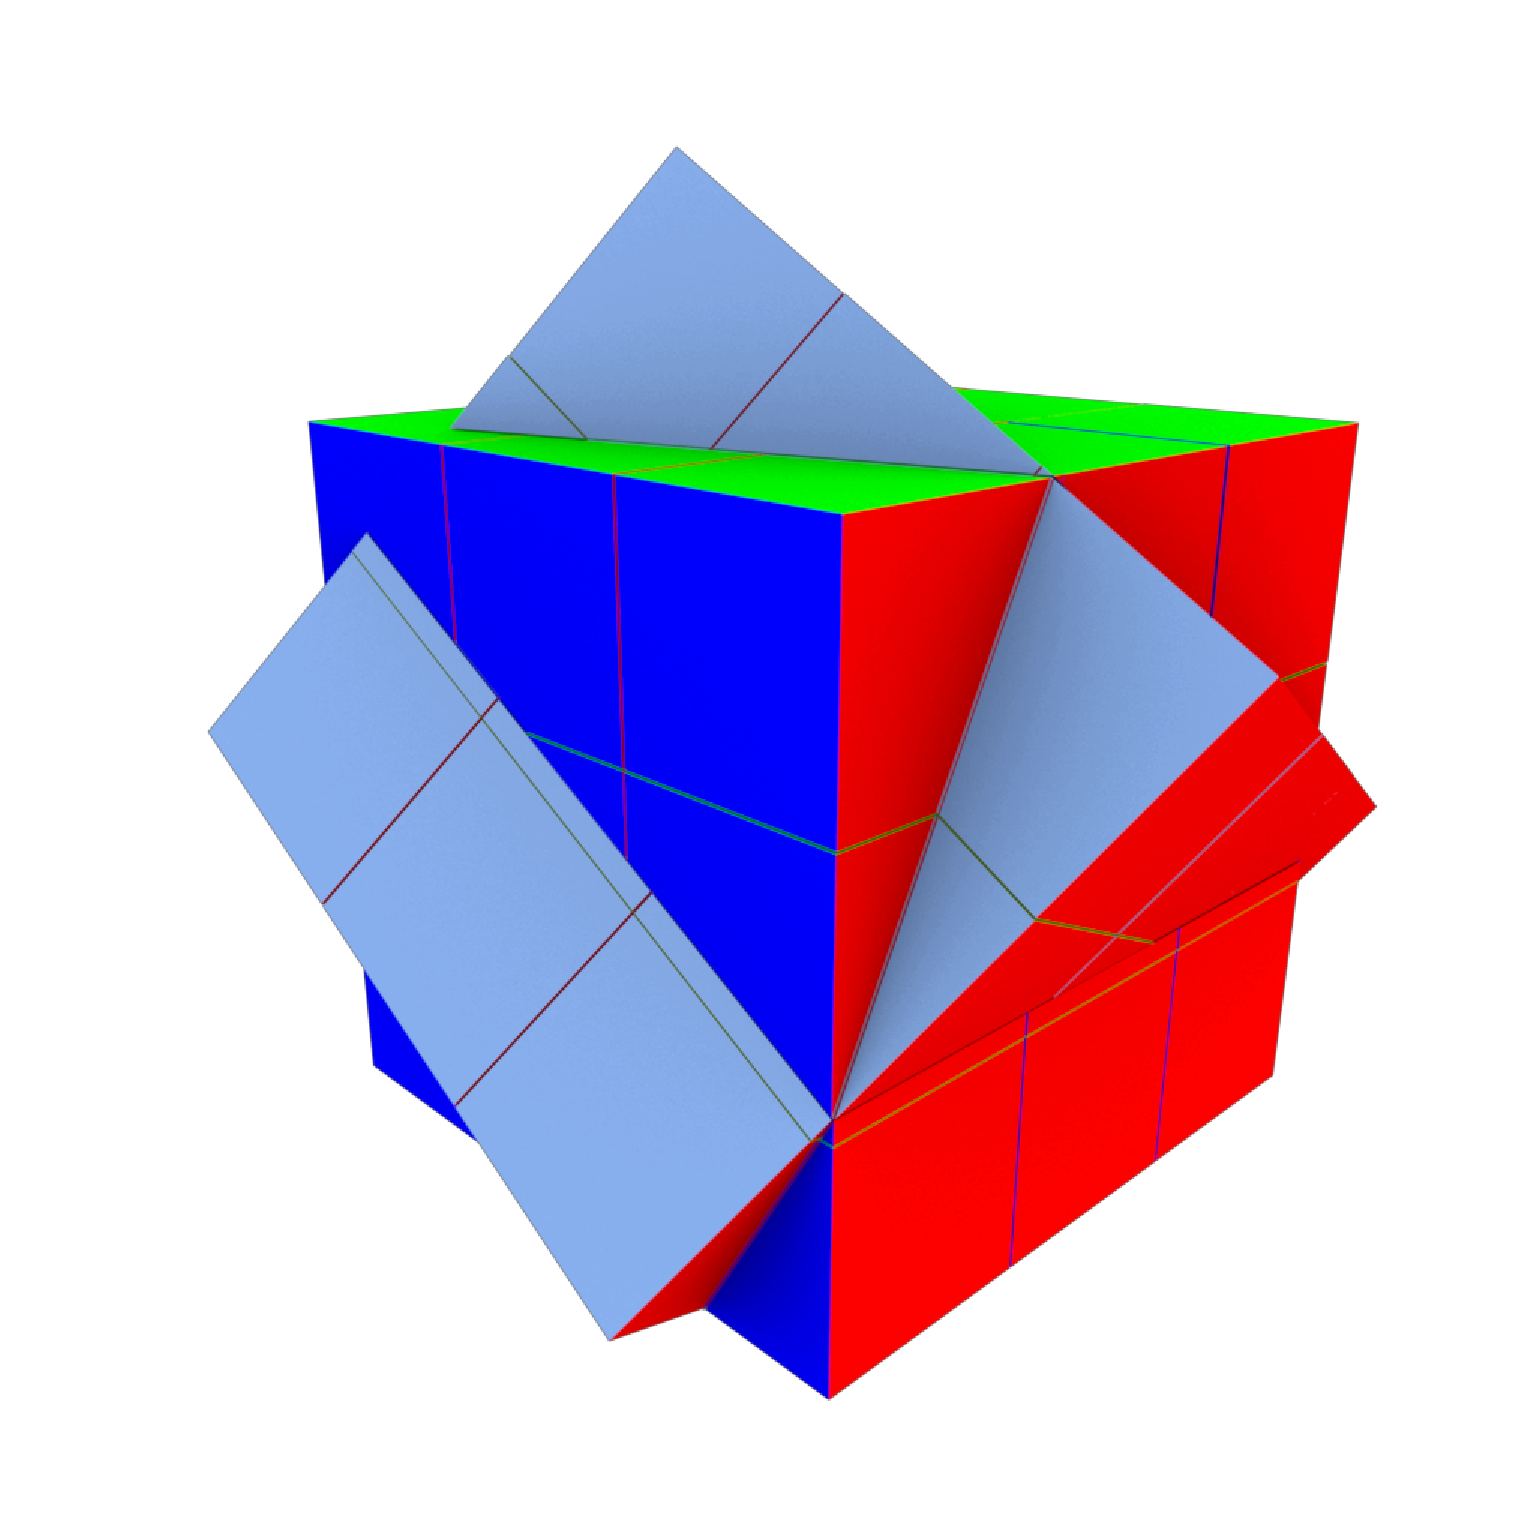
\includegraphics[width=\textwidth]{./img/test-0.pdf}%
    \caption{Input}
\end{figure}

\begin{figure}[h]
    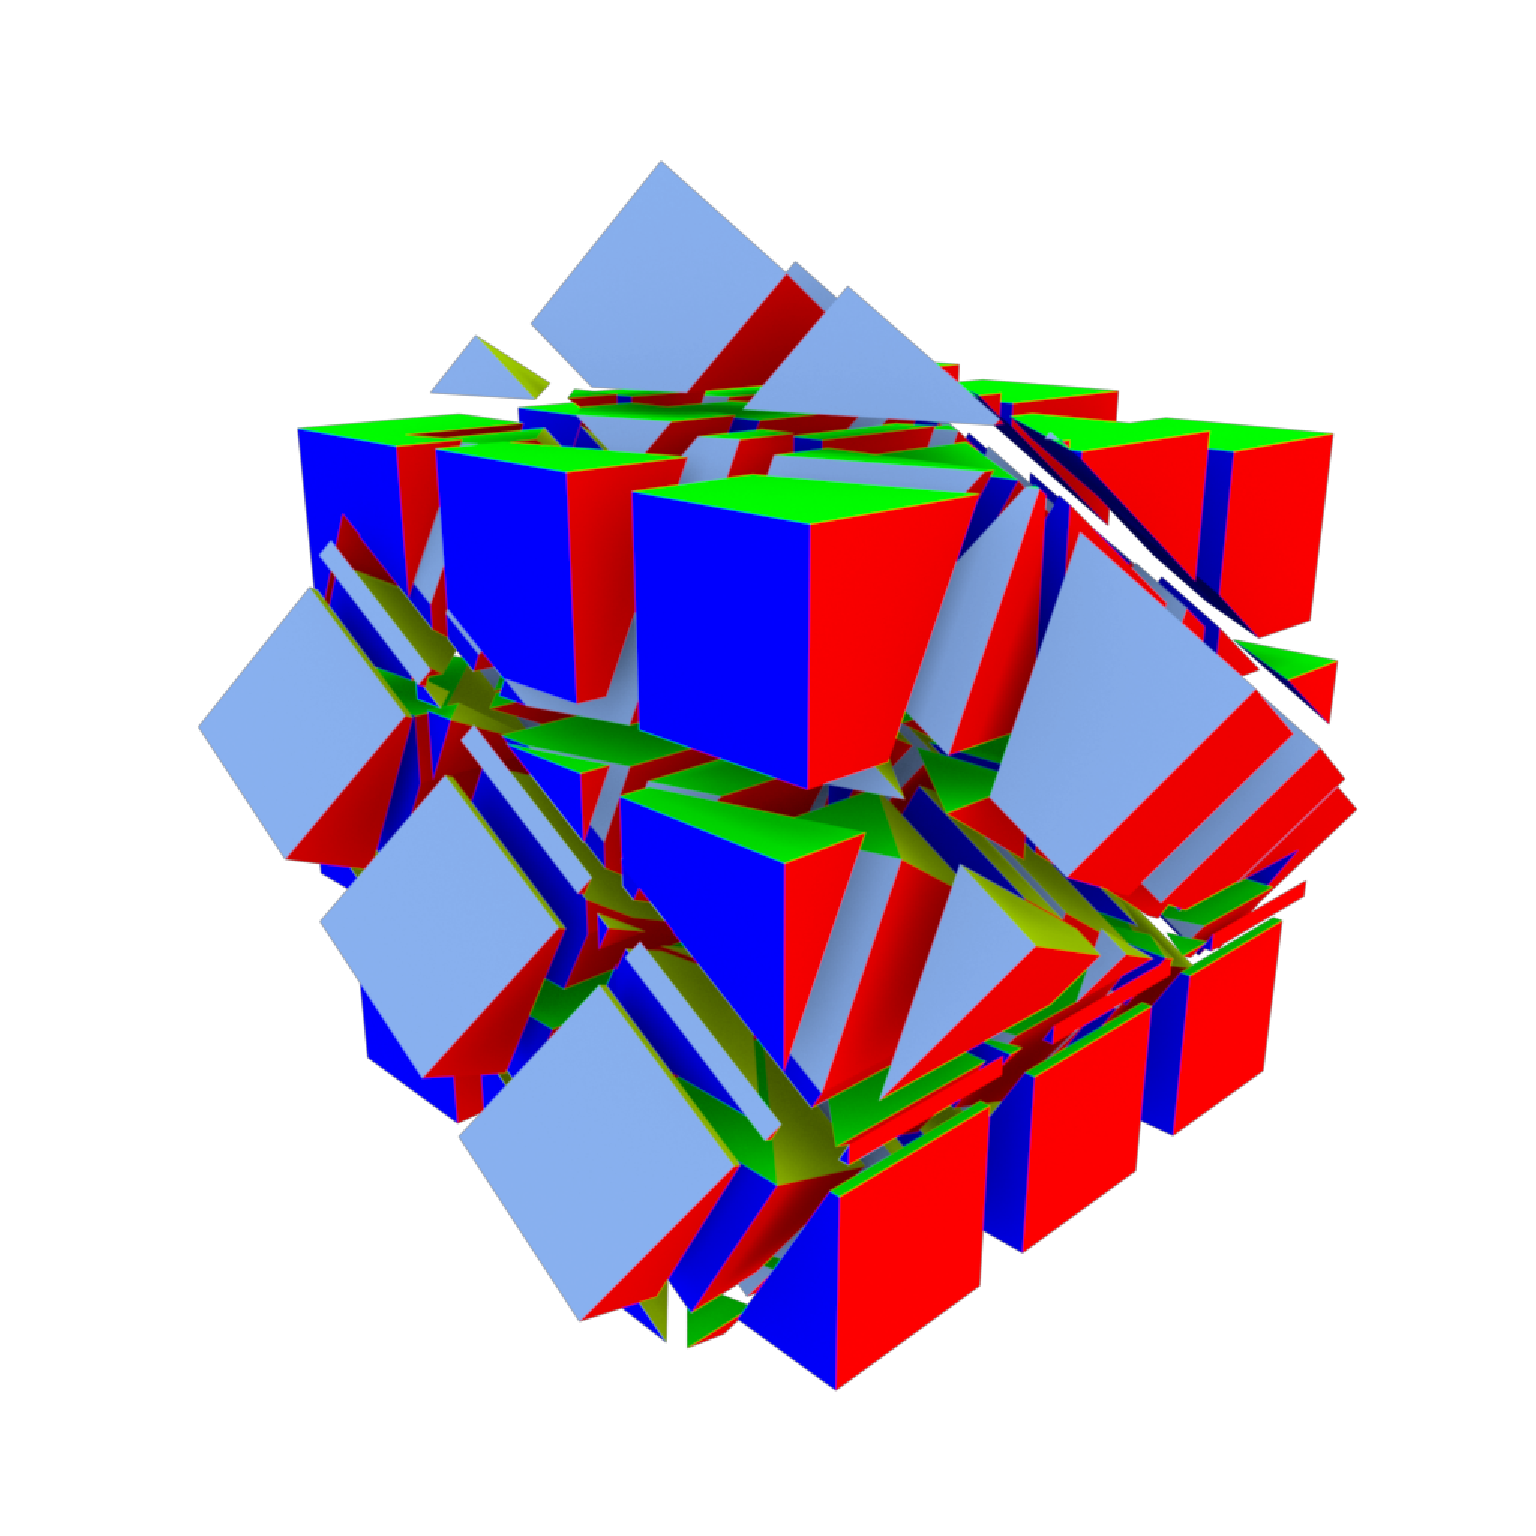
\includegraphics[width=\textwidth]{./img/test-1.pdf}%
    \caption{Output (Exploded)}
\end{figure}

\begin{figure}[h]
    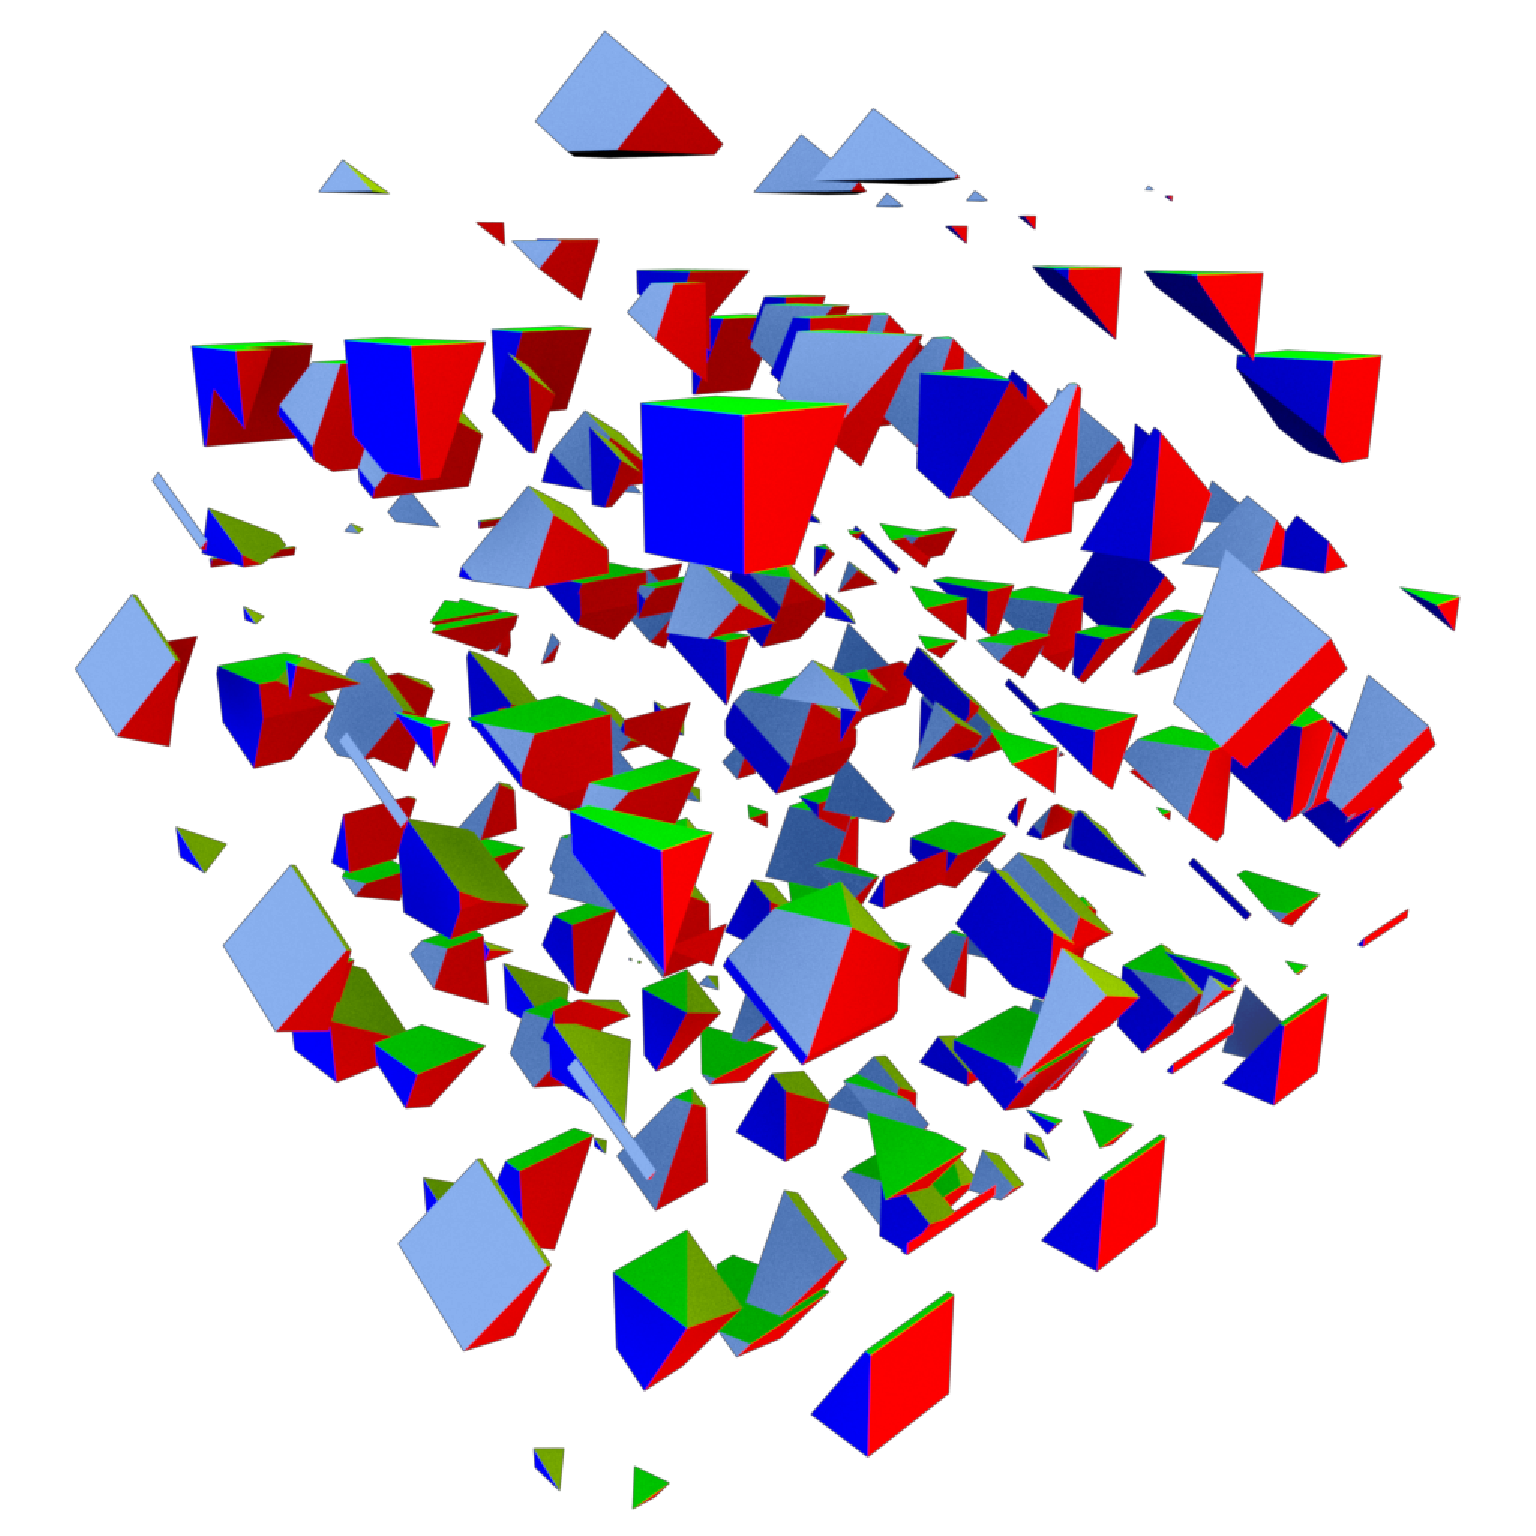
\includegraphics[width=\textwidth]{./img/test-2.pdf}%
    \caption{Output (More exploded)}
\end{figure}